\documentclass[a4paper,12pt]{quantumarticle}
\pdfoutput=1

\usepackage{lipsum}

\title{Example use of rsmf}

\author{Johannes Jakob Meyer}

\begin{document}
\maketitle

\lipsum[1-3]

\begin{figure}
	\centering
	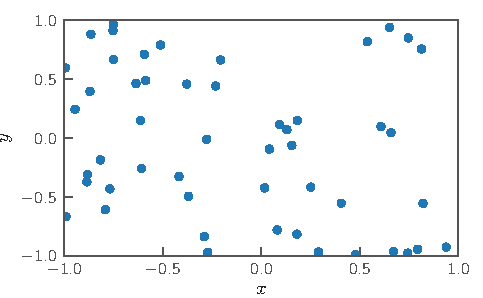
\includegraphics{scatter}
	\caption{This is a very unfancy scatterplot. But consider the size of $x$ and $y$ in the figure above -- they are the same as in the text here. The axes labels are in a smaller fontsize: {\footnotesize 0.0}}
\end{figure}

\lipsum[11-16]

\begin{figure*}
	\centering
	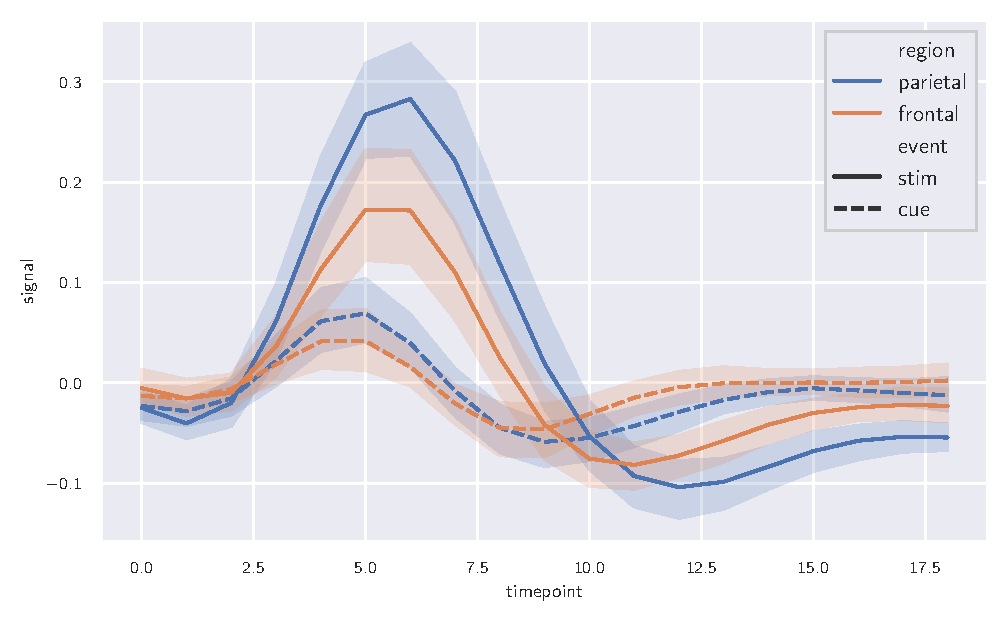
\includegraphics{fmri}
	\caption{\lipsum[1-2]}
\end{figure*}

\lipsum[21-26]

\begin{figure}
	\centering
	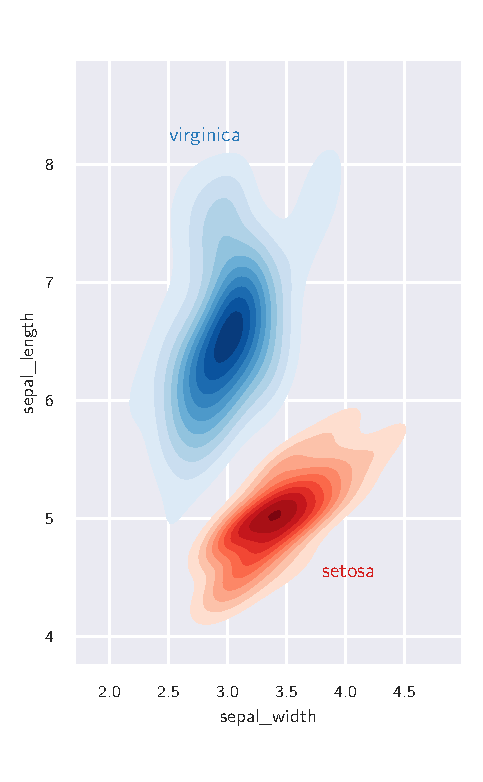
\includegraphics{iris}
	\caption{\lipsum[3]}
\end{figure}

\lipsum[40-44]
    
\end{document}